% !TeX root = ../main-presentation.tex
\begin{frame}
    \frametitle{What are we going to be talking about?}
    \pause
    \centering
    \LARGE
    Digital circuits!

    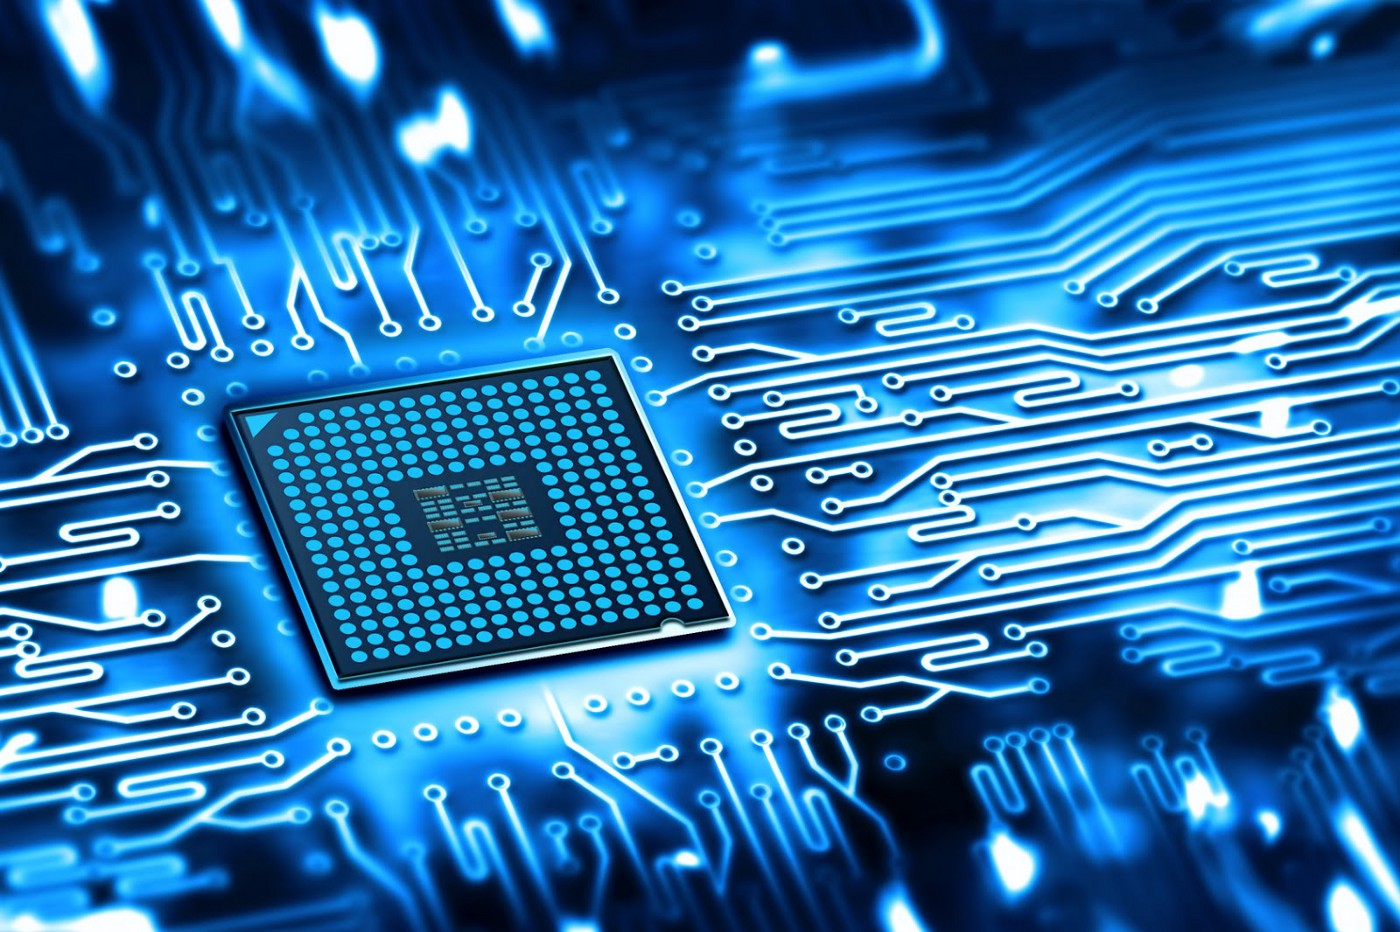
\includegraphics[width=0.6\textwidth]{imgs/circuit}
\end{frame}
\begin{frame}
    \frametitle{What are we going to be talking about?}
    \centering
    \LARGE
    Digital circuits!

    \vspace{1em}
    \normalsize

    \scalebox{2}{\tikzfig{circuits/examples/sr-latch/real-circuit}}
\end{frame}
\begin{frame}
    \frametitle{What are we going to be talking about?}

    \pause

    \centering
    \LARGE
    We want a \alert{compositional} theory of digital circuits.

    \vspace{0.5em}

    \normalsize

    \pause
    \includesvg{imgs/f}
    \pause
    \quad
    \includesvg{imgs/g}
    \pause
    \quad
    \includesvg{imgs/h}

    \pause
    \vspace{1em}

    \raisebox{2em}{\includesvg{imgs/seq}}
    \quad
    \includesvg{imgs/par}
    \quad
    \raisebox{2em}{\includesvg{imgs/trace}}

\end{frame}
\begin{frame}
    \frametitle{But why do we want that?}
    \centering
    \LARGE
    We want to reason \alert{equationally} about circuits.

    \normalsize
    \vspace{2em}

    \pause

    \svg{-0.5}{0.5}{f}
    \quad
    \pause
    \(=\)
    \quad
    \svg{-2}{0.5}{rewrite-l}
    \quad
    \pause
    \(\rightsquigarrow\)
    \quad
    \svg{-2}{0.5}{rewrite-r}
    \quad
    \pause
    \(=\)
    \quad
    \svg{-0.5}{0.5}{g}

\end{frame}
\begin{frame}
    \frametitle{Why all the pictures?}
    \centering

    \Huge

    \only<3>{
        \svg{0}{1.25}{string-crossed}
        \[F \seq \sigma \seq \id \tensor G \seq \sigma \seq H\]
    }%
    \only<4->{
        \svg{0}{1.25}{string-uncrossed}
        \[F \seq G \tensor \id \seq H\]
    }%

\end{frame}
\begin{frame}
    \frametitle{What came before}

    \pause
    \alert{Lafont (2003)}
    \emph{`Towards an algebraic theory of Boolean circuits'}

    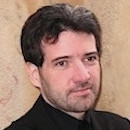
\includegraphics[width=0.15\textwidth]{imgs/lafont}

    \vspace{0.5em}
    \pause

    \alert{Ghica, Jung, Lopez (2017)}
    \emph{`Diagrammatic semantics for digital circuits'}

    \includegraphics[width=0.15\textwidth]{imgs/ghica}
    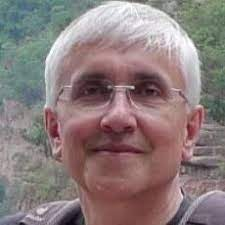
\includegraphics[width=0.15\textwidth]{imgs/achim}
    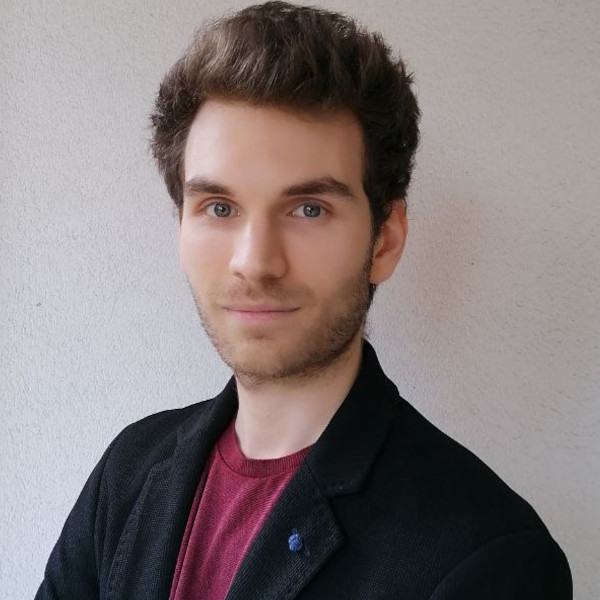
\includegraphics[width=0.15\textwidth]{imgs/lopez}
\end{frame}

\begin{frame}
    \frametitle{Joint work with...}
    \centering
    \begin{minipage}{0.4\textwidth}
        \centering

        \includegraphics[width=0.75\textwidth]{ghica}

        \vspace{0.5em}

        \alert{Dan Ghica}

        University of Birmingham
    \end{minipage}
    \qquad
    \begin{minipage}{0.4\textwidth}
        \centering
        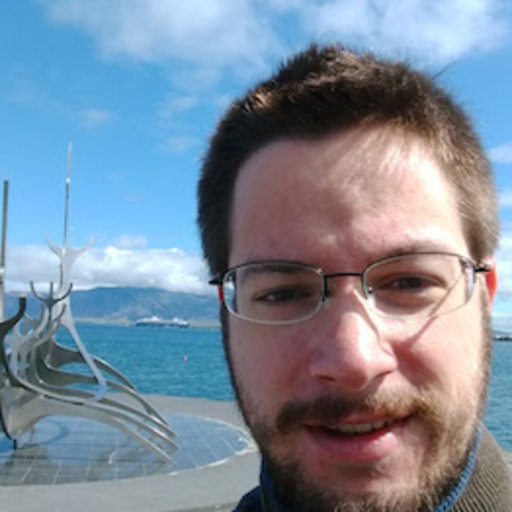
\includegraphics[width=0.75\textwidth]{sprunger}

        \vspace{0.5em}

        \alert{David Sprunger}

        Indiana State University
    \end{minipage}
\end{frame}